\subsection{L5: From Environmental Adaptation to Meta-Improvement}
\label{sec:l5-meta-improvement}

An improvement process can become a bottleneck in its own right. A coding agent may repeatedly generate similar unsuccessful patches because its search procedure discards useful alternatives. A research agent may optimize a development score after that score has stopped predicting external performance. Repairing such failures requires changes to the procedures that direct experiments and judge their outcomes. Designing these procedures is costly: a revision must be assessed through the later improvements it produces, often across several tasks and repeated runs~\cite{zelikman2024stop,shi2026aevolvetraining}.

\textbf{L5 begins when AI persistently modifies a mechanism responsible for future improvements and uses the revised mechanism in subsequent rounds.} The editable mechanism may be an improver, a successor evaluator, a search policy, or a procedure for directing research. L2 searches for candidate interventions; L3 determines what experience to acquire; L4 incorporates deployment feedback into persistent adaptation. L5 additionally makes the procedure governing later improvement an object of improvement. A deployed agent that retains new debugging skills through an unchanged learning procedure exemplifies L4. Revising and reusing the procedure that diagnoses failures and builds those skills can cross the L5 boundary.

The loop closes when a revised mechanism returns to govern the generation, evaluation, or selection of later successors. The inherited state includes the accepted code, prompts, evaluators, or research policy, together with evidence used by later revisions. Human designers still establish the overall mission, protected evaluation, editable components, and resource permissions, and may retain veto and deployment authority. Some of these decisions are enforced by fixed infrastructure; they do not require a person to approve every iteration. Figure~\ref{fig:l5-meta-improvement} illustrates how evidence from earlier attempts can guide a revision of the improvement process, which successors then inherit and reuse.

These conditions distinguish \emph{structural L5}, which demonstrates that an AI-directed change persists and controls a later improvement round, from \emph{effective L5}, which demonstrates that the revised mechanism produces or selects better successors under comparable budgets and independent assessment. Self-modifying task code provides insufficient evidence when the process responsible for later revisions remains unchanged. Conversely, an evolved successor evaluator can establish structural L5 even with unchanged task-agent code. Classification therefore applies to the particular mechanism examined. Table~\ref{tab:l5-recursive-ascent} summarizes the loop, inherited state, and external controls of representative systems.

\begin{figure*}[!t]
  \centering
  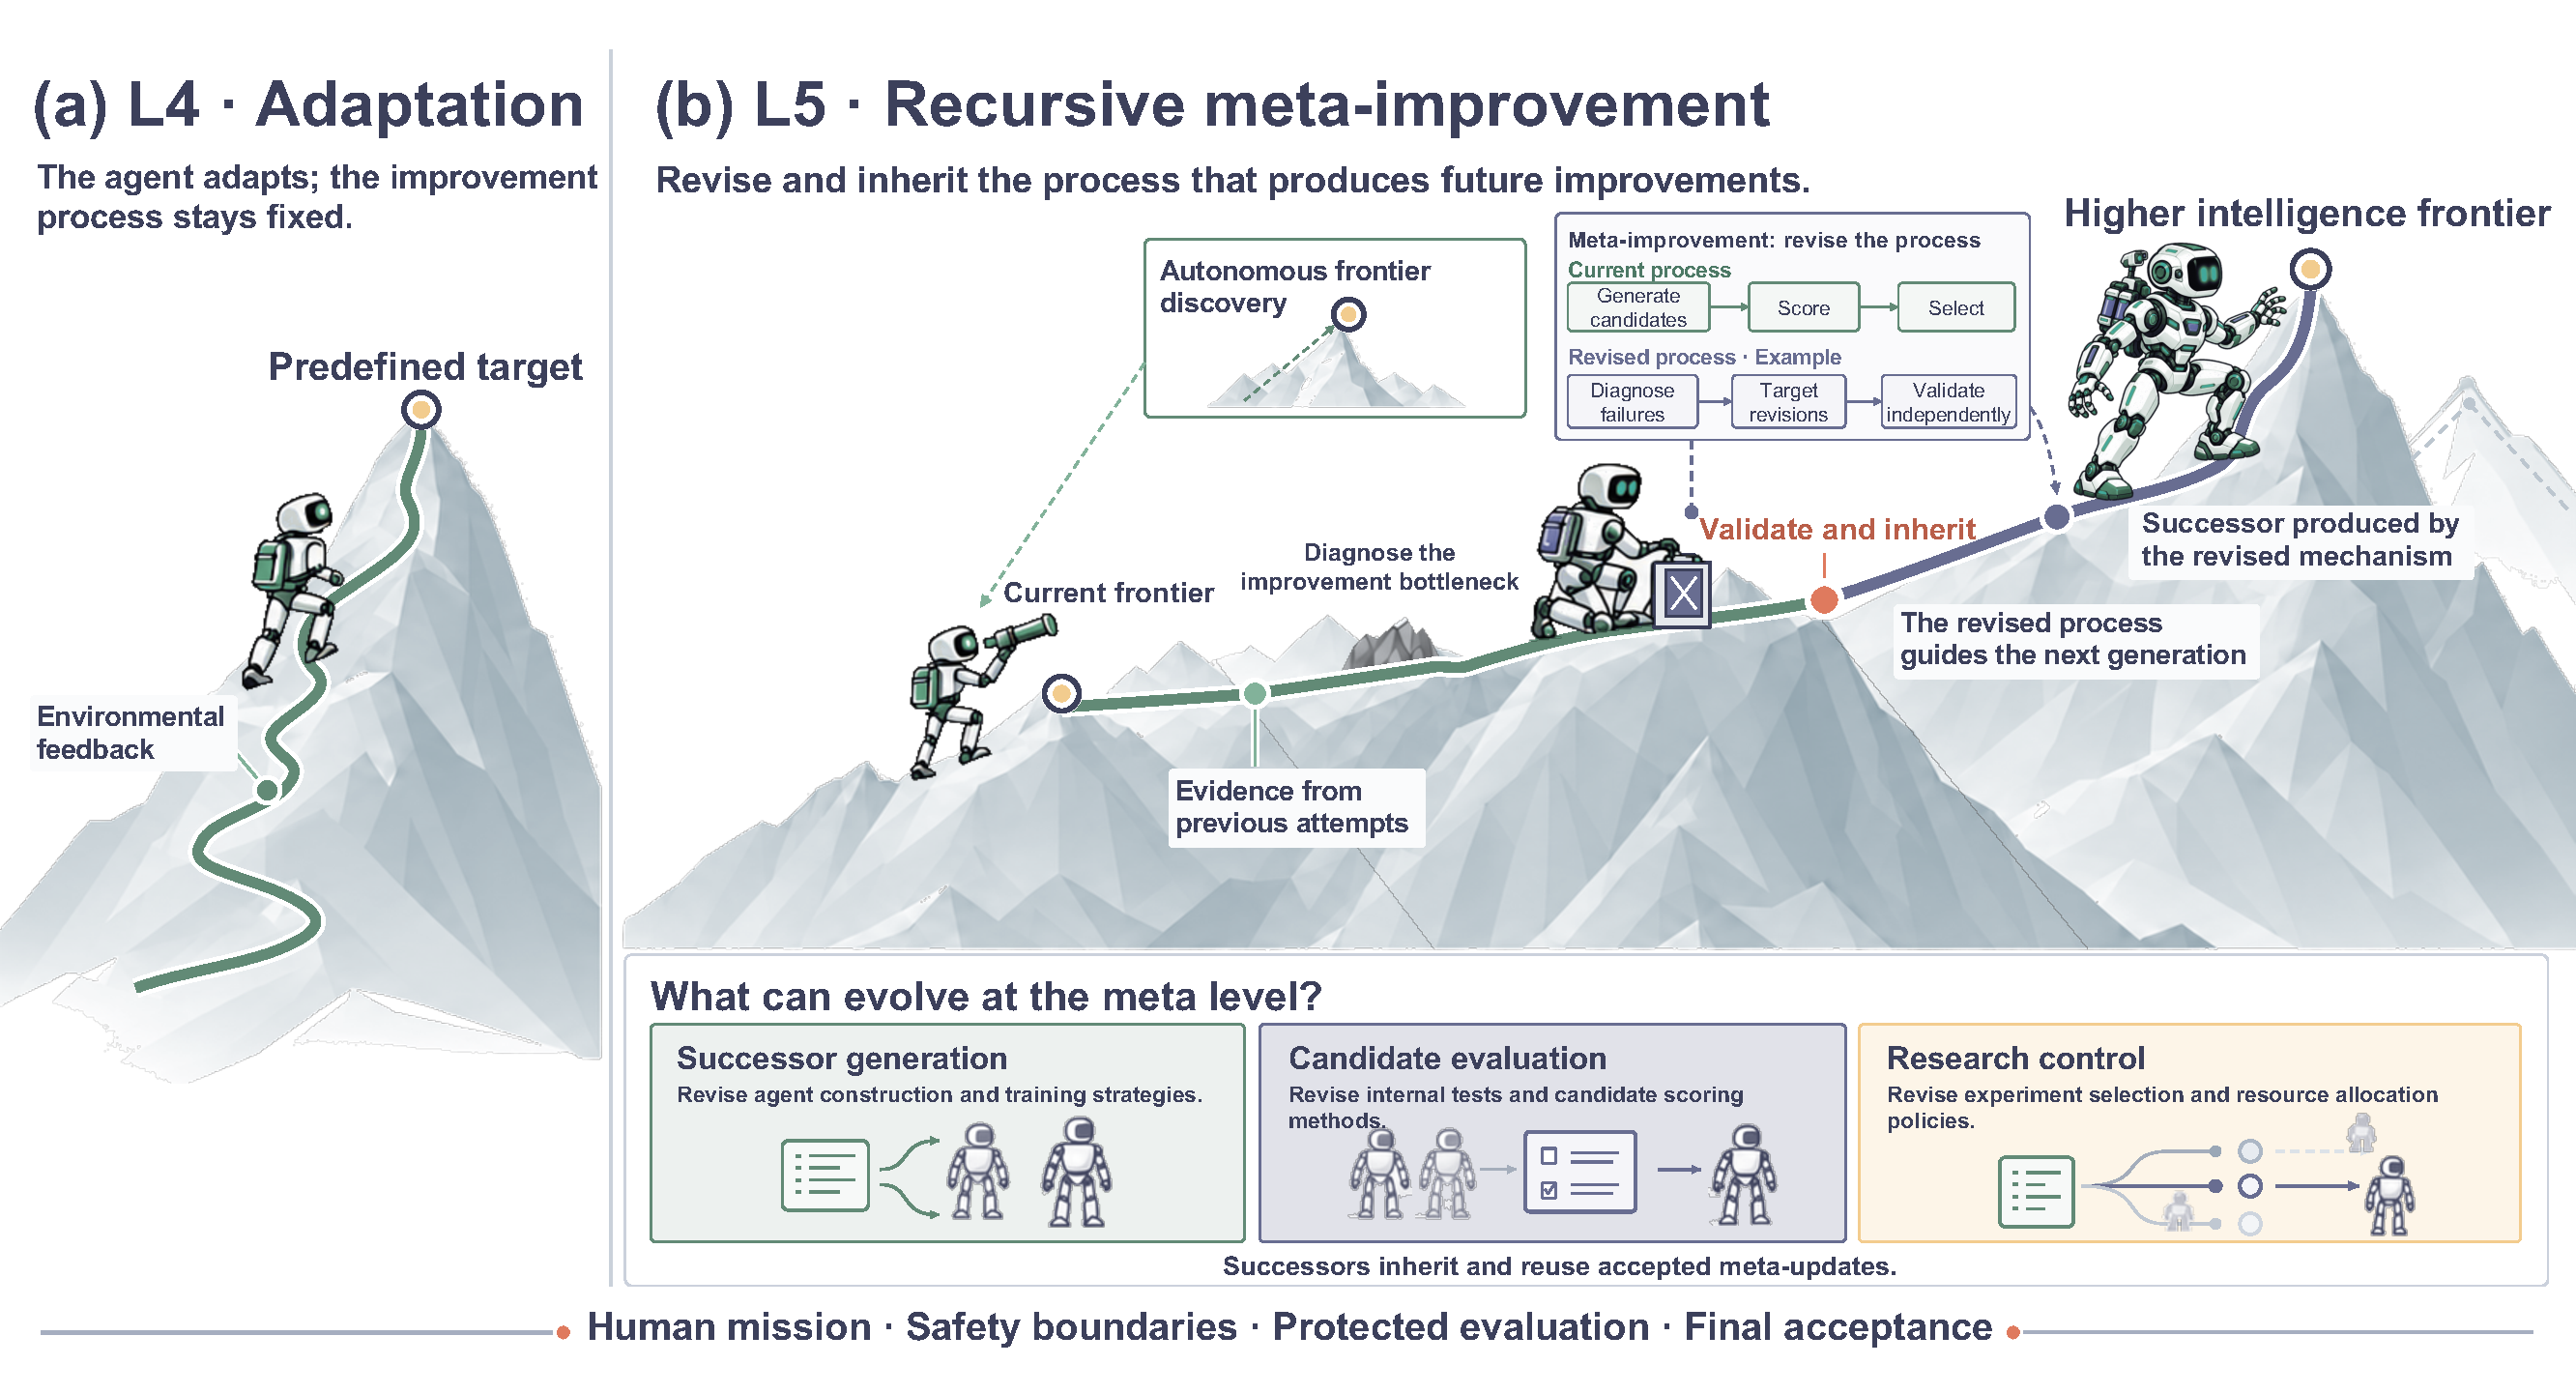
\includegraphics[width=\linewidth]{figures/L5.pdf}
  \caption{From environmental adaptation to recursive meta-improvement. (a) L4 incorporates environmental feedback within a fixed improvement process. (b) L5 diagnoses limitations of that process, revises it, and passes validated changes to successors. Meta-updates can affect successor generation, candidate evaluation, or research control. Human-defined missions, safety boundaries, protected evaluation, and final acceptance remain external constraints. The ascending path illustrates possible progress through inherited meta-updates.}
  \label{fig:l5-meta-improvement}
\end{figure*}

\begin{table*}[t]
  \centering
  \caption{L5 mechanisms and external controls.}
  \label{tab:l5-recursive-ascent}
  \scriptsize
  \setlength{\tabcolsep}{3pt}
  \renewcommand{\arraystretch}{1.12}
  \renewcommand{\tabularxcolumn}[1]{m{#1}}
  \begin{tabularx}{\textwidth}{@{}>{\raggedright\arraybackslash}m{0.19\textwidth}>{\raggedright\arraybackslash}m{0.23\textwidth}>{\raggedright\arraybackslash}m{0.24\textwidth}>{\raggedright\arraybackslash}X@{}}
    \toprule
    \textbf{Work} & \textbf{Loop closes at} & \textbf{Inherited state} & \textbf{External controls} \\
    \midrule
    \multicolumn{4}{@{}l}{\textbf{Search and self-revision}} \\
    STOP~\cite{zelikman2024stop} & Next program search & Improver code & Utility; base LM; budget \\
    \addlinespace[2pt]
    G\"odel Agent~\cite{yin2025godelagent} & Next self-revision & Task and update code & Task objective; runtime access \\
    \addlinespace[2pt]
    DGM~\cite{zhang2026dgm} & Descendant search & Agent code; archive & Parent selection; benchmark \\
    \addlinespace[2pt]
    HyperAgents~\cite{zhang2026hyperagents} & Next agent generation & Task and meta-agent code & Main-study selection; evaluation \\
    \midrule
    \multicolumn{4}{@{}l}{\textbf{Successor evaluation}} \\
    RQGM~\cite{iacob2026redqueen} & Next-epoch selection & Evaluator; agent code & Anchor; replacement schedule \\
    \midrule
    \multicolumn{4}{@{}l}{\textbf{Research policies and harnesses}} \\
    A-Evolve-Training~\cite{shi2026aevolvetraining} & Next research round & Search policy; discovery log & Constitution; benchmark; substrate \\
    \addlinespace[2pt]
    AIRA$_2$~\cite{hambardzumyan2026aira2} / AAR~\cite{chen2026automatedresearchers} & Task experiments & Research artifacts & Research harness; evaluation \\
    \addlinespace[2pt]
    AIDE$^{2}$~\cite{weco2026aide2} & Later research runs & Research-agent harness & Private scores; cost budget \\
    \bottomrule
  \end{tabularx}
  \par\vspace{3pt}{\scriptsize\raggedright\textit{Note:} L5 claims are qualified in the text.\par}
\end{table*}

\subsubsection{Improving the Search Procedure}
\noindent\textbf{The AI revises how future candidate improvements are generated and explored.} A fixed optimizer can spend its budget on unproductive proposals, even when its underlying model can generate better search algorithms. The challenge is to evaluate a proposed optimizer through its ability to improve other programs.

STOP~\cite{zelikman2024stop} makes this problem executable. Its improver is a Python program that calls a fixed language model, generates candidate code, evaluates a supplied utility, and returns a selected candidate. The current improver receives its own source as the optimization target. Successor improvers are scored by the quality of programs they produce on downstream tasks, and the selected improver performs the next self-improvement round. The inherited artifact is thus a search procedure that may introduce beam search, alternative sampling, or other candidate-selection logic. The study reports that a selected fourth-generation improver outperformed the seed on all five transfer tasks excluded from self-improvement. The task distribution, utility, base model, and resource limits remained externally specified. Weaker-model runs regressed on average, and some generated programs evaded soft budgets or exploited evaluation bugs.

G\"odel Agent~\cite{yin2025godelagent} gives the AI access to both its task policy and recursive update logic in a shared Python program. Execution feedback informs a rewrite, and the revised program runs in the next recursive call, including its modified self-update procedure. This broadens the search beyond a developer's fixed editing routine. It also makes errors inheritable: the study reports that 14 of 100 MGSM optimization trials ended below the initial policy's performance, and unrestricted runs could call stronger models. Task objectives and execution permissions therefore remain consequential external controls.

The Darwin G\"odel Machine (DGM)~\cite{zhang2026dgm} retains coding-agent variants and explores their descendants, but keeps archive management and parent selection outside self-modification. Its lineage provides a transition case; task gains alone do not establish a better improvement procedure. HyperAgents~\cite{zhang2026hyperagents} directly exposes both task-agent and meta-agent code to revision. Evolved meta-agents build performance trackers and persistent memory to guide later modifications. In its preprint, meta-agents evolved on paper review and robotics generated improved agents for previously unseen mathematics grading, supporting transfer of the improvement procedure itself. The longer, 200-iteration experiment did not establish a statistically significant final advantage for transferred initialization. Parent selection and evaluation also remained fixed in the main experiments.

\subsubsection{Improving Successor Evaluation}
\noindent\textbf{The AI improves the evaluator that determines which successors are retained.} Repeated optimization places pressure on a judge's blind spots. Keeping that judge unchanged can favor proposals that exploit its errors. Unrestricted judge revision creates the opposite problem: successive scores may reflect changing standards.

The Red Queen G\"odel Machine (RQGM)~\cite{iacob2026redqueen} addresses this tension through evaluator co-evolution. Its learned evaluator remains frozen within an epoch. At a scheduled boundary, challenger evaluators are compared against an independent ground-truth anchor; the selected evaluator then governs the next epoch. Scores dependent on the replaced evaluator are discarded and affected agents are re-evaluated when revisited. The loop carries forward an improved evaluator and agent code while resetting incompatible evaluation records. On held-out Polyglot coding tasks, the preprint reports a 71.7\% pass rate against 69.9\% for HGM-H, with lower search-token use. The anchor, replacement schedule, and orchestration remain externally fixed. These controls preserve a reference against which evaluator changes can be judged; the formal stability argument applies within each frozen epoch, not to unrestricted changes of objective.

\subsubsection{Revising Research Goals and Policies}
\noindent\textbf{The AI uses accumulated experimental evidence to revise what later research should pursue.} Choosing a higher target is difficult when the available proxy rewards progress on the wrong bottleneck. In model post-training, testing that hypothesis requires comparing training runs, identifying failed search directions, and deciding whether to revise the research policy itself. A changing curriculum reaches L5 when its persistent selection procedure is also revised and reused.

A-Evolve-Training~\cite{shi2026aevolvetraining} provides a concrete case. Its preprint reports autonomous post-training of a 30B model across four rounds. Workers return recipe changes, checkpoint evaluations, and failures; a collector consolidates these results, and a meta-agent revises the next round's search policy. The policy carries a standing recipe, promoted or retired search directions, and a registry of unsuccessful approaches. When development scores increased without corresponding external gains, the revised policy directed workers toward interventions that could improve the external target despite lowering the proxy. The study reports a final leaderboard score of 0.86, compared with 0.87 for the top human submission. Cross-round inheritance resides in the research policy and discovery log; the underlying worker substrate and constitution remain fixed. The case supports policy-level L5 within a human-defined objective, with no demonstrated autonomous revision of that objective.

A spiral of improvement emerges when an inherited procedure helps expose a new limitation and is revised again to address it. The next goal should identify a testable capability gap, preserve established capabilities, and justify further expenditure. Goal revision alone supplies limited evidence: the evaluation must establish that the revised policy changes subsequent research and improves its outcomes.

\subsubsection{Industrial Practice}
Industrial implementations expose different portions of the improvement process to revision. Their relevance to L5 depends on whether the retained artifact changes later research decisions.

\emph{Research infrastructure.} Meta's AIRA$_2$~\cite{hambardzumyan2026aira2} uses asynchronous experimentation and hidden consistent evaluation; Anthropic's Automated Alignment Researchers~\cite{chen2026automatedresearchers} generate and test mitigations for specified alignment failures. These systems automate experiment execution within researcher-designed workflows. Their reported results concern research outputs, without establishing inherited changes to the procedures conducting the research.

\emph{Research-agent revision.} Weco's AIDE$^{2}$~\cite{weco2026aide2} applies a research agent to improving a research-agent harness. Candidate harnesses run downstream tasks under private scoring and a fixed cost budget. Accepted versions are retained for subsequent research; a separate experiment installs an evolved harness as the outer improver. Weco reports seven accepted improvements over 100 unattended steps and transfer to external tasks. Its stronger test of whether the evolved agent improves the outer search faster found no statistically significant efficiency advantage. These company-reported results support bounded harness improvement. Private evaluation, task families, and cost constraints remain human-designed, while reliable acceleration of successive improvers remains unestablished.

Across these configurations, the potential saving comes from reusing a better research procedure. Evidence of reduced human development effort requires accounting for the work spent designing evaluators, investigating failures, and maintaining the evolved code. Task performance or unattended runtime alone cannot quantify that saving.

\subsubsection{Evaluating L5 Recursive Improvement}
Evaluation must distinguish a stronger current agent from a procedure that reliably produces stronger successors. SEA-Eval~\cite{jiang2026sea} and SEAGym~\cite{zheng2026seagym} contribute trajectory-based assessment: performance across rounds, held-out transfer, retention, and resource use. Table~\ref{tab:l5-evaluation} summarizes these measurements and the additional mechanism tests needed for L5.

\begin{table*}[!t]
  \centering
  \caption{Evaluating recursive improvement.}
  \label{tab:l5-evaluation}
  \scriptsize
  \setlength{\tabcolsep}{3pt}
  \renewcommand{\arraystretch}{1.12}
  \renewcommand{\tabularxcolumn}[1]{m{#1}}
  \begin{tabularx}{\textwidth}{@{}>{\raggedright\arraybackslash}m{0.14\textwidth}>{\raggedright\arraybackslash}m{0.48\textwidth}>{\raggedright\arraybackslash}X@{}}
    \toprule
    \textbf{Dimension} & \textbf{Measurements} & \textbf{Purpose} \\
    \midrule
    Adaptivity & Gain; improvement trajectory; time to target~\cite{jiang2026sea,zheng2026seagym} & Detect progress and plateaus \\
    \addlinespace[2pt]
    Retention & Replay loss; tasks fixed or broken~\cite{zheng2026seagym} & Detect displaced capabilities \\
    \addlinespace[2pt]
    Transfer & Held-out gains within and across domains~\cite{zheng2026seagym} & Test reuse beyond update tasks \\
    \addlinespace[2pt]
    Efficiency & Tokens; time; cost per validated gain~\cite{jiang2026sea,zheng2026seagym} & Account for improvement expense \\
    \addlinespace[2pt]
    Stability & Harmful updates; largest temporary decline~\cite{jiang2026sea,zheng2026seagym} & Expose unreliable trajectories \\
    \addlinespace[2pt]
    Meta-recursion & Mechanism reuse; successor quality~\cite{zelikman2024stop,zhang2026hyperagents,iacob2026redqueen}; goal and stopping decisions & Test inherited improvement capacity \\
    \bottomrule
  \end{tabularx}
  \par\vspace{3pt}{\scriptsize\raggedright\textit{Note:} Trajectory measures synthesize the cited benchmarks. The meta-recursion row adds our L5 tests: cited systems illustrate mechanism reuse and improvement capacity; goal selection and stopping remain evaluation requirements.\par}
\end{table*}

A mechanism audit should identify the revised artifact, record the evidence that motivated it, and verify its invocation in a later improvement round. To establish effectiveness, the original and revised mechanisms should start from comparable agents and evidence under matched budgets, including the cost of evaluating the mechanisms. Holding the revised mechanism fixed during transfer tests helps isolate what it learned about improvement. HyperAgents~\cite{zhang2026hyperagents} uses this design to distinguish transferable agent-generation ability from performance on the original task.

Goal selection needs complementary evaluation. Adaptive frontier tasks can test whether the system identifies useful next challenges; protected reference tasks preserve comparability and expose forgetting or reward hacking. Private tasks with previously undisclosed rules strengthen tests of discovery beyond familiar distributions. Evaluations should also record whether the system stops when expected benefit falls below cost or risk. These are proposed requirements for assessing fuller L5 autonomy, rather than capabilities established by existing RSI benchmarks.

Current results support bounded meta-improvement: accepted changes to improvers, evaluators, or research policies can govern subsequent rounds, and some changes transfer across tasks~\cite{zelikman2024stop,zhang2026hyperagents,iacob2026redqueen}. Statistically reliable accumulation across generations under comparable resources remains open~\cite{zhang2026hyperagents,weco2026aide2}. The practical objective is to increase validated improvement per unit of computation and human effort. Strong base models, execution infrastructure, and independent evaluation continue to supply the resources and constraints under which that improvement occurs.

\begin{center}
\fbox{
\parbox{0.92\linewidth}{
\textbf{Finding: L5 makes the improvement procedure inheritable.}
The loop closes through reuse of a revised improver, evaluator, or research policy. Successors inherit that procedure and its supporting evidence; humans retain the overall objective, protected acceptance criteria, and resource authority.
}}
\end{center}
